\documentclass[journal]{IEEEtrancz}
% zvolte kodovani
\usepackage[utf8]{inputenc} % linux/unix
%\usepackage[latin2]{inputenc}
%\usepackage[cp1250]{inputenc} % Windows
\usepackage[czech]{babel}
\usepackage{graphicx}

\begin{document}

\title{Semestrální práce předmětu a0m33eoa - TSP s několika cestujícími}
\author{Jakub Moravec}

\maketitle

\begin{abstrakt}
Zde uvést krátky odstavec s abstraktem. V abstraktu stručně shrnuto o čem článek je.
Čtenář je motivován, proč by měl článek číst, poslední věta zpravidla.
shrnuje dosažené výsledky.
\end{abstrakt}

\IEEEpeerreviewmaketitle

\section{Zadání}
Úkolem je vyřešit úlohu TSP s několika cestujícími pomocí evolučního algoritmu. Na vstupu je úplný neorientovaný graf o \textit{N} uzlech. Cílem je nalézt takovou množinu cest pro \textit{M} cestujících, které všechny vychází z počátečního uzlu (depotu) a zase v něm končí, všechny uzly (kromě depotu) jsou navštíveny právě jednou a délka nejdelší cesty je minimální. Žádná z cest nesmí mít nulovou délku.

\section{Úvod}
Úloha TSP s několika cestujícími známá také jako \textbf{VRP} (\textit{Vehicle routing problem}) je kombinatorická optimalizační úloha odpovídající otázku "Jaké je optimální uspořádání hran pro několik cestujicích tak, aby byly výsledné cesty pokrývající všechny uzly nejkratší?". Určení optimálního řešení tohoto problému je \textit{NP-těžká} úloha, proto bývá částo řešena pomocí heuristik a aproximačních algoritmů. V tomto dokumentu budou představena řešení pomocí \textit{lokálního prohledávání}, \textit{evolučního algoritmu} a \textit{memetického algoritmu} (kombinace předcházejících). 

% fitness fce
\textit{Fiteness funkce} pro vyhodnocování optimality řešení byla převzata ze zadání úlohy: kvalita řešení je určena jako délka nejdelší cesty z M cest. Tuto fitness funkci se budeme snažit minimalizovat.

% reprezentace
Jako reprezentace řešení problému byla zvolena uspořádaná množnina identifikátorů měst, kde pořadí měst určuje pořadí jejich průchodu. Depot (id 0) je v množině obsažen \textit{M +1} krát, všechna ostatní města právě jednou. Tato reprezentace byla zvolena proto, aby bylo možné stejným způsobem použitými algoritmy měnit pořadí měst v cestách jednotlivých cestovatelů i přesouvat města mezi cestovateli.  

\section{Cíl práce}
Cílem práce je implementovat \textit{algoritmus lokálního prohledávání}, \textit{evolučníh algoritmus} a \textit{memetický algoritmus} generující řešení problému taková, aby jejich hodnota fitness funkce byla minimální a to při co možná nejmenším počtu vyhodnocení definované fitness funkce. 

%TODO
\section{Experimenty}
V této sekci budou představeny všechny implementované algoritmy a jejich výsledky. 

%TODO basic pseudocode

%TODO společné prvky
% turnajová selekce
% 

\subsection{Algoritmus lokálního prohledávání}
% mutace?
% crossover? 

\subsection{Evoluční algoritmus}
% selection crossover 
% simple mutace

\subsection{Memetický algoritmus}
% upravená mutace
% selection crossover
% dva local search - picking podle úspěšnosti
% local searche provádějí analýzu na základě modelu, nenavyšují počet vyhodnocení fitness

% TODO tabulka s parametry - společné versus speciální pro jednotlivé přístupy

% TODO grafy fitness dle počtu ohodnocení / epoch 

% TODO souhrnná tabulka

% TODO obrázky nejhezčích řešení

\begin{figure}[ht]
  \centering
    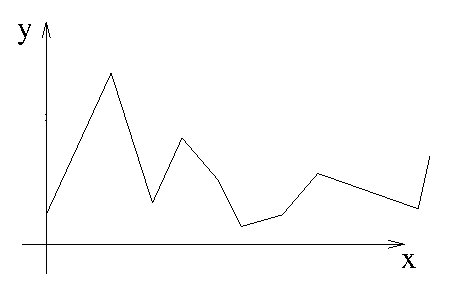
\includegraphics{figure}
      \caption{Název a stručný popis obrázku}
    \label{fig:exfig}
\end{figure}

Do experimetální části se přímo hodí obrázky. Každý obrázek musí být řádně vysvětlen
a okomentován. U grafů musí být popsány osy, pod obrázek umístíme název a 
krátké vysvětlení toho, co na obrázku je. Obrázek \ref{fig:exfig} je příklad
umístění obrázku do dokumentu.

\begin{table}
  \centering
  \caption{Parametry experimentu}
  \begin{tabular}{|l||c|c|c|}
  \hline
    & A & B & C \\
  \hline
  \hline
  S učitelem  & 0.22 & 0.27 & 0.29 \\
  \hline
  Bez učitele & 0.12 & 0.17 & 0.20 \\ 
  \hline
  \end{tabular}
  \label{tab:extab}
\end{table}

Výsledky experimentu je vhodné shrnout tabulkou, příkladem
je tabulka \ref{tab:extab}. Pro tabulku platí totéž co 
pro obrázek s výjimkou toho, že popis a název tabulky je nad tabulkou. Z tabulky
musí být jasné, co je jejím obsahem. Vysvětlení obsahu je vhodné uvést 
do textu poblíž tabulky.

\section{Diskuse}
Referát na tento předmět by neměl být větší než 3 strany v tomto formátu. 
Vlastní text by měl obsahovat úvod do problematiky zkoumaných dat, jejich rozbor. Návrh
použité neuronové sítě a v tabulce přehledné vstupní nastavení experimentu. Vždy je vhodné
uvést příklad zkoumaných dat, jaké obsahují atributy apod. Diskuse je důležitá kapitola,
která rozebírá dosažené výsledky. 

\section{Závěr}
Každý článek/referát musí obsahovat závěr, který stručně shrnuje dosažené výsledky 
experimentů. Závěr neobsahuje žádná nová zjištění, která by předtím v textu nebyla rozvedena.
Závěr je nejdůležitější část článku. Na základě závěru zpravidla pokrařujeme ve čtení
publikace. 

\end{document}
